In diesem Schritt wollen wir nun die Untersuchungen aus 
\nameref{ch:Content2:sec:APosteriori} durchführen. Nach dem Rendern eines
$Frames_{t}$(vor dem Rendern von $Frame_{t+1}$) approximieren wir das Histogramm
der Pixelwerte anhand der Pixelwerte von $Frame_{t}$. Dabei betrachten wir
Anzahl Pixel pro BLOCK in der unmittelbaren Nachbarschaft und nehmen diese
wie anfangs erwähnt als Schätzung des Histogramms.

\cite{hal02158423}
\begin{algorithm}[H]
    \caption{\textbf{Sortier Schritt t} nach dem Rendern von Frame t
    und vor dem Rendern von Frame t+1}
    \begin{algorithmic}[1]
        \State pixel \textbf{consists of} value,index;
        \State List framePixelsIntensities, noiseIntensities;
        \State $assert(sizeof(framePixelsIntensities)==BLOCKSIZE)$;
        \State $assert(sizeof(noiseIntensities)==BLOCKSIZE)$;
        \State List L $\leftarrow$ pixels of frame t in block;
        \State \hfill
        \State //init lists
        \State initList(framePixelsIntensities, pixelIntensity(L);
        \State $blueNoise_{t}$ = calcCorrectOffset(incomingbluenoisetexture);
        \State initList(noiseIntensities, pixelIntensity($blueNoise_{t}$));
        \State \hfill
        \State //sort the two lists by means of intensities
        \State sort(framePixelsIntensities);
        \State Sort(noiseIntensities);
        \State \hfill
        \State //now we reorder our seeds hence the sorted lists
        \For{$i = 1 .. BLOCKSIZE$}
        \State $sortedSeeds(noiseIntensities.getIndex(i)) = incomingSeeds(framePixelIntensities.getIndex(i))$;
        \EndFor
    \end{algorithmic}
    \label{alg:Sortier}
\end{algorithm}

Hierbei muss noch eine wichtige Anmerkung gemacht werden. Die Fehlerverteilung
der Pixelwerte im Bildraum konvergiert auf diese Weise nicht zu einer 
blue noise Verteilung. Wir wechseln in jedem Frame die 
verwendeten blue noise Texturen um gewissen Artefakten zu entgehen und 
andere temporale Algorithmen zu ermöglichen. Dieser Schritt alleine reicht
also nicht für den erwünschten Effekt.

\begin{figure}[H]

    \begin{subfigure}{\textwidth}
        \centering 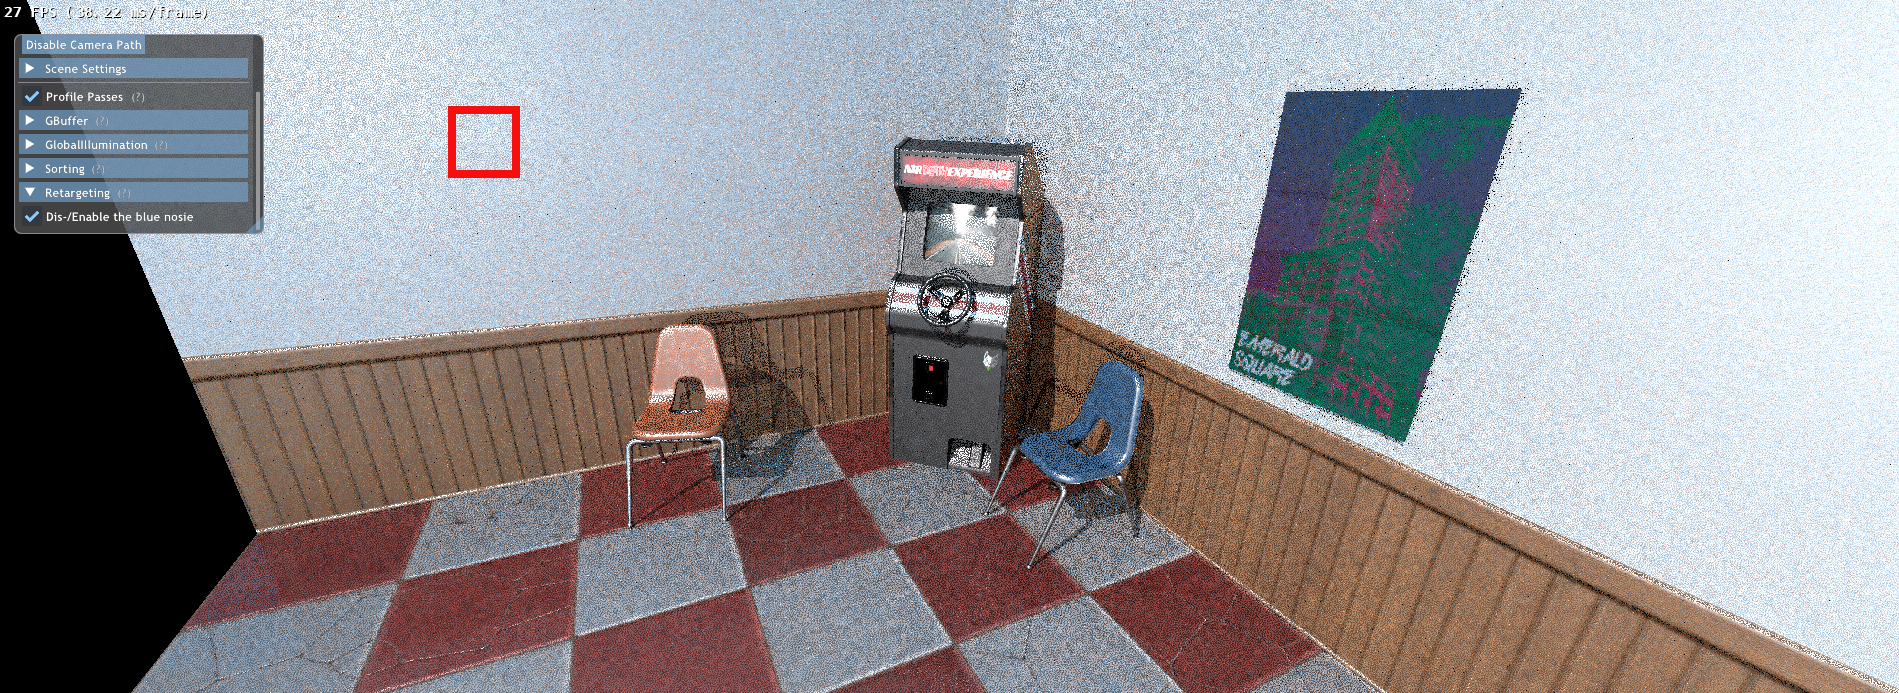
\includegraphics[scale=.2]{content/TemporalerAlg/Bilder/blue_noise_sorting.png}
        \caption{Szene}
        \label{fig:Szene_white_noise}
    \end{subfigure}
    \begin{subfigure}{0.5\textwidth}
        \centering 
\includegraphics[width=0.5\linewidth]{content/TemporalerAlg/Bilder/blue_noise_sorting_64x64.jpg} 
        \caption{Szenenausschnitt}
        \label{fig:ausschnitt_white_noise}
    \end{subfigure}
    \begin{subfigure}{0.5\textwidth}
        \centering 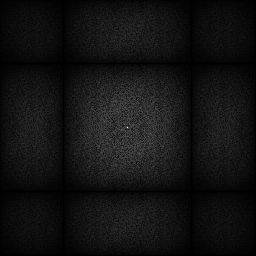
\includegraphics[width=0.5\linewidth]{content/TemporalerAlg/Bilder/blue_noise_sorting_64x64_fourier.png}
        \caption{Fouriertransformierte des Ausschnitts}
        \label{fig:Fouriertransformierte_blue_noise_sorting}
    \end{subfigure}
        \caption{Path Tracer nur Sorting}
        \label{fig:blue noise szene}
\end{figure}